% distinct products in the N x N table (generated by a script).
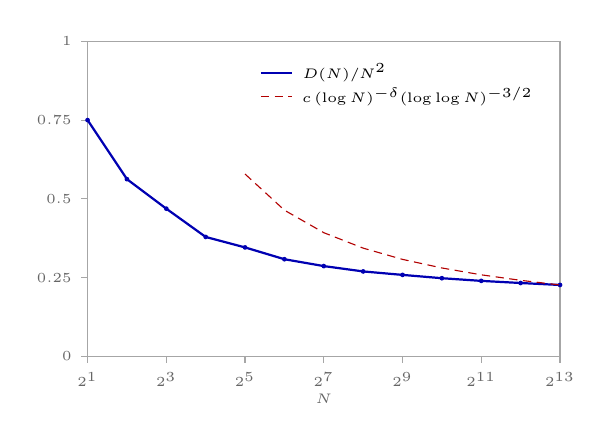
\begin{tikzpicture}[x=1cm,y=1cm]
\draw[black!35] (0,0) rectangle (6.00,4.00);
\draw[black!35] (0.00,0)--(0.00,-0.08) node[below,font=\tiny,black!60]{$2^{1}$};
\draw[black!35] (1.00,0)--(1.00,-0.08) node[below,font=\tiny,black!60]{$2^{3}$};
\draw[black!35] (2.00,0)--(2.00,-0.08) node[below,font=\tiny,black!60]{$2^{5}$};
\draw[black!35] (3.00,0)--(3.00,-0.08) node[below,font=\tiny,black!60]{$2^{7}$};
\draw[black!35] (4.00,0)--(4.00,-0.08) node[below,font=\tiny,black!60]{$2^{9}$};
\draw[black!35] (5.00,0)--(5.00,-0.08) node[below,font=\tiny,black!60]{$2^{11}$};
\draw[black!35] (6.00,0)--(6.00,-0.08) node[below,font=\tiny,black!60]{$2^{13}$};
\draw[black!35] (0,0.00)--(-0.08,0.00) node[left,font=\tiny,black!60]{$0$};
\draw[black!35] (0,1.00)--(-0.08,1.00) node[left,font=\tiny,black!60]{$0.25$};
\draw[black!35] (0,2.00)--(-0.08,2.00) node[left,font=\tiny,black!60]{$0.5$};
\draw[black!35] (0,3.00)--(-0.08,3.00) node[left,font=\tiny,black!60]{$0.75$};
\draw[black!35] (0,4.00)--(-0.08,4.00) node[left,font=\tiny,black!60]{$1$};
\node[below,font=\tiny,black!60] at (3.00,-0.35) {$N$};
\draw[blue!70!black,thick] (0.000,3.000) -- (0.500,2.250) -- (1.000,1.875) -- (1.500,1.516) -- (2.000,1.383) -- (2.500,1.233) -- (3.000,1.146) -- (3.500,1.078) -- (4.000,1.034) -- (4.500,0.992) -- (5.000,0.958) -- (5.500,0.931) -- (6.000,0.906);
\fill[blue!70!black] (0.000,3.000) circle (0.03cm);
\fill[blue!70!black] (0.500,2.250) circle (0.03cm);
\fill[blue!70!black] (1.000,1.875) circle (0.03cm);
\fill[blue!70!black] (1.500,1.516) circle (0.03cm);
\fill[blue!70!black] (2.000,1.383) circle (0.03cm);
\fill[blue!70!black] (2.500,1.233) circle (0.03cm);
\fill[blue!70!black] (3.000,1.146) circle (0.03cm);
\fill[blue!70!black] (3.500,1.078) circle (0.03cm);
\fill[blue!70!black] (4.000,1.034) circle (0.03cm);
\fill[blue!70!black] (4.500,0.992) circle (0.03cm);
\fill[blue!70!black] (5.000,0.958) circle (0.03cm);
\fill[blue!70!black] (5.500,0.931) circle (0.03cm);
\fill[blue!70!black] (6.000,0.906) circle (0.03cm);
\draw[red!70!black,densely dashed] (2.000,2.315) -- (2.500,1.856) -- (3.000,1.570) -- (3.500,1.374) -- (4.000,1.231) -- (4.500,1.122) -- (5.000,1.035) -- (5.500,0.965) -- (6.000,0.906);
\draw[blue!70!black,thick] (2.20,3.60)--(2.60,3.60) node[right,font=\tiny,black]{$D(N)/N^2$};
\draw[red!70!black,densely dashed] (2.20,3.30)--(2.60,3.30) node[right,font=\tiny,black]{$c\,(\log N)^{-\delta}(\log\log N)^{-3/2}$};
\end{tikzpicture}
